Neste anexo será apresentado como o desenvolvedor poderá implementar uma
aplicação paralela sobre a adaptação proposta do \fw \pskel. Na adaptação o desenvolvedor
terá que implementar o código sobre o \fw \pskel para os processos mestre e
trabalhador. Como pode-se analisar no código~\ref{cod:jacobiMestreA}, o
desenvolvedor terá que implementar a função \texttt{main} com as estruturas
providas pelo \fw. Primeiramente, o desenvolvedor irá declarar matrizes de
entrada e saída (linhas 4 e 5), onde $A$ é
a matriz de entrada, $M$ e $N$ são as dimensões de largura e altura
respectivamente e $B$ é a matriz de saída. Para especificar a máscara da computação, o desenvolvedor deve determinar quais
vizinhos serão utilizados, de forma genérica, por meio de posições relativas à
célula central (linha 6). Mais especificamente, a Figura~\ref{fig:stencilA} ilustra uma
possível configuração de vizinhos, onde temos as posições: \texttt{\{-1,0\}}
para a célula à esquerda, \texttt{\{0,1\}} para a célula superior,
\texttt{\{0,-1\}} para a célula inferior e \texttt{\{1,0\}} para a célula à
direita. Após a caracterização dos vizinhos, será definida a máscara da
computação por meio da abstração proveniente do \fw (linha 7). A estrutura
\texttt{Arguments} (linha 8) será responsável por enviar ao \textit{Kernel} da
computação variáveis auxiliares definidas pelo desenvolvedor. Desta forma, o
desenvolvedor precisa definir uma \texttt{struct} manualmente e passar como
parâmetro para a estrutura
principal do \fw, denominada \texttt{Stencil}. A estrutura \texttt{Stencil}
apresenta configurações \texttt{1D}, \texttt{2D} e \texttt{3D}. Na declaração da
estrutura, o desenvolvedor irá determinar as matrizes de entrada e saída

\begin{figure}[!h]
    \centering
    \caption{Esquemático ilustrando possíveis vizinhos em uma computação \stencil.}
    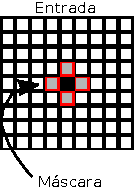
\includegraphics[width=3cm]{figs/vizinhosAnexo.pdf} \\
    Fonte: Desenvolvido pelo autor.
    \label{fig:stencilA}
\end{figure}

\begin{figure}[!h]
    \begin{lstlisting}[
        caption=Exemplo de código de uma aplicação genérica no processo mestre.,
        label=cod:jacobiMestreA,
        ]
  int main(int argc, char **argv) {
      /* variaveis omitidas */

      Array2D<float> input(A, M, N);
      Array2D<float> output(B, M, N);
      int neighbors = {{x,y}, {x,y}, ...};
      Mask2D<int> mask(neighbors.size(), neighbors);
      struct Arguments args(alpha);

      Stencil2D<Array2D<float>, Mask2D<int>, Arguments>
          application(A, B, mask, args);
      application.scheduleMPPA(slave_bin, threadsNum, clustersNum,
                               tileDim, iterations);

      return(0);
  }
    \end{lstlisting}
\end{figure}
\begin{figure}[!h]
    \begin{lstlisting}[
        caption=Exemplo de código de uma aplicação genérica no processo trabalhador.,
        label=cod:jacobiTrabalhadorA,
        ]
  __parallel__ void
  stencilKernel(Array2D<float> A, Array2D<float> B, Mask2D<int> mask,
  struct Arguments args, int x, int y){
      B(x,y) = /* Kernel determinado pelo desenvolvedor */
  }

  int main(int argc, char **argv) {
      /* variaveis omitidas */

      Array2D<float> inputTile(A, M, N);
      Array2D<float> outputTile(B, M, N);
      int neighbors = {{x,y}, {x,y}, ...};
      Mask2D<int> mask(neighbors.size(), neighbors);
      struct Arguments args(alpha);

      Stencil2D<Array2D<float>, Mask2D<int>, Arguments>
          application(A, B, mask, args);
      application.runMPPA(cluster_id, numThreads, numTiles,
                          iterations);

      return(0);
  }
    \end{lstlisting}
\end{figure}

utilizadas, a máscara da computação e a estrutura de argumentos (linhas 10 e 11). Por fim, a
estrutura \texttt{Stencil} possui um método de gerenciamento para o \mppa,
denominado \texttt{scheduleMPPA}, responsável por realizar o particionamento de
dados e comunicação (linhas 12 e 13). Esse método será chamado passando como parâmetros: o nome
do binário do processo trabalhador\footnote{O nome do binário é determinado pelo desenvolvedor.}, o
número de \textit{threads} e \textit{clusters} definidos pelo usuário, a dimensão
dos \textit{tiles} e o número de iterações sobre a aplicação.


Para o processo trabalhador, o desenvolvedor terá que implementar a função \texttt{main}
de forma similar. Contudo, o método de gerenciamento é diferente, onde
o desenvolvedor irá chamar o método de execução para o \textit{cluster} do \mppa,
denominado \texttt{runMPPA}, passando o identificador do \textit{cluster}, o número de \textit{threads},
número de \textit{tiles} que serão enviados pelo processo mestre e o número de iterações
(linhas 18 e 19). As informações sobre o número de \textit{tiles}, largura ($M$),
altura ($N$), identificador do \textit{cluster}, número de \textit{threads} e
iterações são enviadas pelo processo mestre e obtidos pelos argumentos
da função \texttt{main}. Por fim, o desenvolvedor terá que implementar a computação da aplicação, isto é,
o \textit{Kernel} \stencil da aplicação (linhas 1-5). O \textit{Kernel}, geralmente, utiliza
elementos da matriz de entrada ($A$), realiza operações sobre esse elemento de
acordo com os vizinhos caracterizados pela máscara da computação e atribui o
resultado à matriz de saída ($B$) na posição respectiva. Além disso, a computação
recebe como parâmetro a estrutura de argumentos para utilizar variáveis
auxiliares definidas pelo usuário. Exemplos de aplicações e da
adaptação podem ser encontrados no seguinte link:
\url{https://github.com/pskel/pskel/tree/mppaWidth}.





